\documentclass{extbook}[14pt]
\usepackage{multicol, enumerate, enumitem, hyperref, color, soul, setspace, parskip, fancyhdr, amssymb, amsthm, amsmath, bbm, latexsym, units, mathtools}
\everymath{\displaystyle}
\usepackage[headsep=0.5cm,headheight=0cm, left=1 in,right= 1 in,top= 1 in,bottom= 1 in]{geometry}
\pagestyle{fancy}
\lhead{}
\chead{Answer Key for Module\,6\,-\,Polynomial\,Functions Version A}
\rhead{}
\lfoot{Summer\,C\,2020}
\cfoot{}
\rfoot{}
\begin{document}
\textbf{This key should allow you to understand why you choose the option you did (beyond just getting a question right or wrong). \href{https://xronos.clas.ufl.edu/mac1105spring2020/courseDescriptionAndMisc/Exams/LearningFromResults}{More instructions on how to use this key can be found here}.}

\textbf{If you have a suggestion to make the keys better, \href{https://forms.gle/CZkbZmPbC9XALEE88}{please fill out the short survey here}.}

\textit{Note: This key is auto-generated and may contain issues and/or errors. The keys are reviewed after each exam to ensure grading is done accurately. If there are issues (like duplicate options), they are noted in the offline gradebook. The keys are a work-in-progress to give students as many resources to improve as possible.}

\rule{\textwidth}{0.4pt}

26. Describe the zero behavior of the zero $x = 6$ of the polynomial below.
\[ f(x) = 4(x - 3)^{7}(x + 3)^{6}(x - 6)^{10}(x + 6)^{9} \] 

 
 The solution is  
 \begin{center} 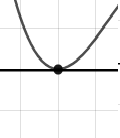
\includegraphics[width=0.3\textwidth]{../Figures/polyZeroBehaviorCA.png} \end{center}\begin{tabular}{|c|c|} 
\hline 
 & \tabularnewline 
 \textbf{A.} 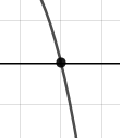
\includegraphics[width=0.3\textwidth]{../Figures/polyZeroBehaviorAA.png} & \textbf{B.} 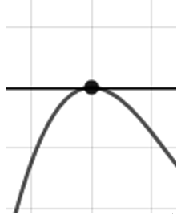
\includegraphics[width=0.3\textwidth]{../Figures/polyZeroBehaviorBA.png} \tabularnewline 
\hline 
 & \tabularnewline 
 \textbf{C.} 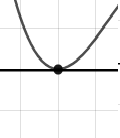
\includegraphics[width=0.3\textwidth]{../Figures/polyZeroBehaviorCA.png} & \textbf{D.} 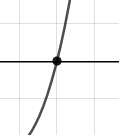
\includegraphics[width=0.3\textwidth]{../Figures/polyZeroBehaviorDA.png} \tabularnewline 
\hline 
 E. None of the figures above. & \tabularnewline 
\hline 
 \end{tabular} 
 
\begin{enumerate}[label=\Alph*.] 
\item   
\item   
\item   
\item   
\end{enumerate} 
 
\textbf{General Comments:} You will need to sketch the entire graph, then zoom in on the zero the question asks about.

-----------------------------------------------

27. Which of the following equations \textit{could} be of the graph presented below?
\begin{center} 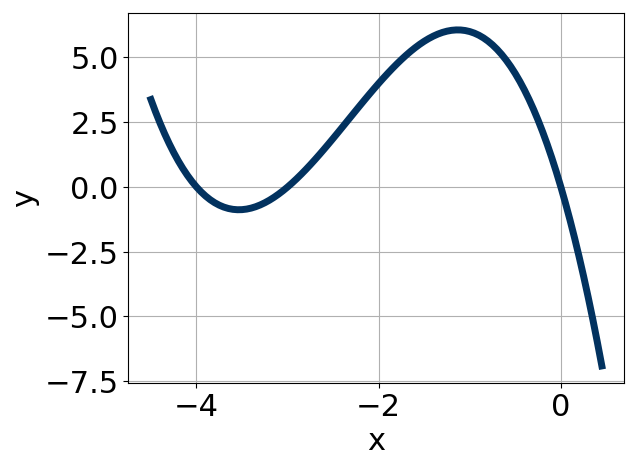
\includegraphics[width=0.3\textwidth]{../Figures/polyGraphToFunctionA.png} \end{center} 

The solution is $ 14x^{8} (x - 1)^{5} (x + 4)^{9} $ 

\begin{enumerate}[label=\Alph*.] 
\item $ 14x^{4} (x - 1)^{6} (x + 4)^{7} $ 

 The factor $(x - 1)$ should have an odd power. 
\item $ 14x^{8} (x - 1)^{5} (x + 4)^{9} $ 

 * This is the correct option. 
\item $ 18x^{5} (x - 1)^{4} (x + 4)^{11} $ 

 The factor $0$ should have an even power and the factor $1$ should have an odd power. 
\item $ -19x^{10} (x - 1)^{11} (x + 4)^{11} $ 

 This corresponds to the leading coefficient being the opposite value than it should be. 
\item $ -9x^{4} (x - 1)^{9} (x + 4)^{8} $ 

 The factor $(x + 4)$ should have an odd power and the leading coefficient should be the opposite sign. 
\end{enumerate} 
 
General Comments: Draw the x-axis to determine which zeros are touching (and so have even multiplicity) or cross (and have odd multiplicity).

-----------------------------------------------

28. Construct the lowest-degree polynomial given the zeros below. Then, choose the intervals that contain the coefficients of the polynomial in the form $x^3+bx^2+cx+d$.
\[ -3 + 2i \text{ and } -1 \] 
The solution is $ x^{3} +7 x^{2} +19 x + 13 $ 

\begin{enumerate}[label=\Alph*.] 
\item $ b \in [-4, 2], c \in [-2, 0], \text{ and } d \in [-6, 1] $ 

 $x^{3} + x^{2} -x -2$, which corresponds to multiplying out $(x -2)(x + 1)$. 
\item $ b \in [-8, -2], c \in [18, 27], \text{ and } d \in [-16, -12] $ 

 $x^{3} -7 x^{2} +19 x -13$, which corresponds to multiplying out $(x-(-3 + 2i))(x-(-3 - 2i))(x -1)$. 
\item $ b \in [4, 9], c \in [18, 27], \text{ and } d \in [4, 14] $ 

 * $x^{3} +7 x^{2} +19 x + 13$, which is the correct option. 
\item $ b \in [-4, 2], c \in [2, 9], \text{ and } d \in [0, 4] $ 

 $x^{3} + x^{2} +4 x + 3$, which corresponds to multiplying out $(x + 3)(x + 1)$. 
\item $ \text{None of the above.} $ 

 This corresponds to making an unanticipated error or not understanding how to use nonreal complex numbers to create the lowest-degree polynomial. If you chose this and are not sure what you did wrong, please contact the coordinator for help. 
\end{enumerate} 
 
General Comments: Remember that the conjugate of $a+bi$ is $a-bi$. Since these zeros always come in pairs, we need to multiply out $(x-(-3 + 2i))(x-(-3 - 2i))(x-(-1))$.

-----------------------------------------------

29. Construct the lowest-degree polynomial given the zeros below. Then, choose the intervals that contain the coefficients of the polynomial in the form $ax^3+bx^2+cx+d$.
\[ 5, \frac{-2}{3}, \text{ and } \frac{-3}{2} \] 
The solution is $ 6x^{3} -17 x^{2} -59 x -30 $ 

\begin{enumerate}[label=\Alph*.] 
\item $ a \in [1, 10], b \in [-19, -11], c \in [-60, -48], \text{ and } d \in [25, 33] $ 

 $6x^{3} -17 x^{2} -59 x + 30$, which corresponds to multiplying everything correctly except the constant term. 
\item $ a \in [1, 10], b \in [-19, -11], c \in [-60, -48], \text{ and } d \in [-33, -29] $ 

 * $6x^{3} -17 x^{2} -59 x -30$, which is the correct option. 
\item $ a \in [1, 10], b \in [32, 40], c \in [17, 20], \text{ and } d \in [-33, -29] $ 

 $6x^{3} +35 x^{2} +19 x -30$, which corresponds to multiplying out $(x + 1)(3x + 3)(2x -2)$. 
\item $ a \in [1, 10], b \in [9, 21], c \in [-60, -48], \text{ and } d \in [25, 33] $ 

 $6x^{3} +17 x^{2} -59 x + 30$, which corresponds to multiplying out $(x + 5)(3x -2)(2x -3)$. 
\item $ a \in [1, 10], b \in [39, 46], c \in [69, 83], \text{ and } d \in [25, 33] $ 

 $6x^{3} +43 x^{2} +71 x + 30$, which corresponds to multiplying out $(x + 1)(3x -3)(2x -2)$. 
\end{enumerate} 
 
General Comments: To construct the lowest-degree polynomial, you want to multiply out $(x -5)(3x + 2)(2x + 3)$

-----------------------------------------------

30. Describe the end behavior of the polynomial below.
\[ f(x) = -7(x - 6)^{3}(x + 6)^{8}(x + 9)^{5}(x - 9)^{6} \] 

 
 The solution is  
 \begin{center} 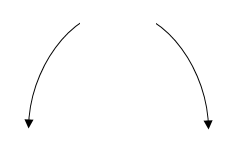
\includegraphics[width=0.3\textwidth]{../Figures/polyEndBehaviorBA.png} \end{center}\begin{tabular}{|c|c|} 
\hline 
 & \tabularnewline 
 \textbf{A.} 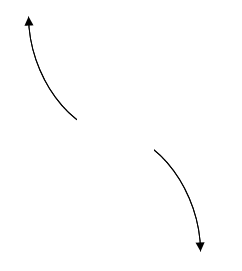
\includegraphics[width=0.3\textwidth]{../Figures/polyEndBehaviorAA.png} & \textbf{B.} 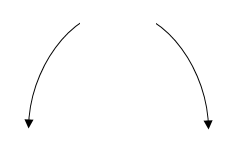
\includegraphics[width=0.3\textwidth]{../Figures/polyEndBehaviorBA.png} \tabularnewline 
\hline 
 & \tabularnewline 
 \textbf{C.} 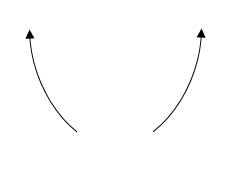
\includegraphics[width=0.3\textwidth]{../Figures/polyEndBehaviorCA.png} & \textbf{D.} 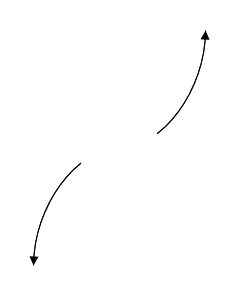
\includegraphics[width=0.3\textwidth]{../Figures/polyEndBehaviorDA.png} \tabularnewline 
\hline 
 E. None of the figures above. & \tabularnewline 
\hline 
 \end{tabular} 
 
\begin{enumerate}[label=\Alph*.] 
\item The function is above the $x$-axis, then passes through.  
\item The function is below the $x$-axis, then touches.  
\item The function is above the $x$-axis, then touches.  
\item The function is below the $x$-axis, then passes through.  
\end{enumerate} 
 
\textbf{General Comments:} Remember that end behavior is determined by the leading coefficient AND whether the \textbf{sum} of the multiplicities is positive or negative.

-----------------------------------------------


\end{document}

